\documentclass{article}
\usepackage{mathtools}
\usepackage{xfrac}
\usepackage{amsfonts}
\usepackage{amsthm}
\usepackage{subfig}
\usepackage{hyperref}
\usepackage{xcolor}

\usepackage{times}
\usepackage{float}

\usepackage{natbib}
\usepackage{nips_2018}

\usepackage{bbm}

\newtheorem{theorem}{Theorem}
\newtheorem{lemma}{Lemma}

\allowdisplaybreaks

\title{Uncertainty propagation in neural networks for sparse coding}

\author{} % LEAVE BLANK FOR ORIGINAL SUBMISSION.
          % UAI  reviewing is double-blind.

% The author names and affiliations should appear only in the accepted paper.
%
%\author{ {\bf Harry Q.~Bovik\thanks{Footnote for author to give an
%alternate address.}} \\
%Computer Science Dept. \\
%Cranberry University\\
%Pittsburgh, PA 15213 \\
%\And
%{\bf Coauthor}  \\
%Affiliation          \\
%Address \\
%\And
%{\bf Coauthor}   \\
%Affiliation \\
%Address    \\
%(if needed)\\
%}

%\author{ {\bf Danil Kuzin} \\
%\And
%{\bf Olga Isupova}  \\
%\And
%{\bf Lyudmila Mihaylova}   \\
%}

\begin{document}

\maketitle

\begin{abstract}
In the Bayesian neural network framework prior distributions are imposed on weights of a network and a posterior distribution of an output is inferred, rather than a point prediction provided by conventional neural networks. Therefore, Bayesian neural networks estimate both an output for a test data and uncertainty of this prediction. Uncertainty of the prediction is a result of weight uncertainty propagation through the layers of a network. We propose a novel method of propagating uncertainty through the soft thresholding nonlinearity. The method expands the area of Bayesian neural networks and enables the soft thresholding nonlinearity to be included in Bayesian deep neural networks for the first time. As an example we design a Bayesian Learned Iterative Shrinkage-Thresholding Algorithm (Bayesian \textsc{lista}) network. We develop a highly efficient posterior inference algorithm based on probabilistic backpropagation. A series of experiments on sparse coding shows that the proposed framework provides both accurate predictions and quantified estimates of uncertainty in these predictions.
\end{abstract}

\section{Introduction}
Though the idea of Bayesian learning in neural networks is not new \citep{neal2012bayesian}, it has regained its attention recently with the development of distributed approximate inference techniques \citep{li2015stochastic, hoffman2013stochastic}  and general boost in popularity of deep learning. In some spheres, such as self-driving cars or healthcare, uncertainty estimates are very important and Bayesian learning allows to obtain them.

In general, when distributions are included in a network, the complexity of Bayesian inference scales exponentially with the number of layers. Thus, it is infeasible to apply conventional Bayesian inference algorithms for deep neural networks. Nevertheless, recently several techniques have been proposed to handle specific types of neural networks. For example, feed-forward networks with the rectified linear unit nonlinearity~\citep{hernandez2015probabilistic}, networks with discrete distributions~\citep{soudry2014expectation}, recurrent networks~\citep{mcdermott2017bayesian}.

There are currently two approaches in Bayesian neural networks: explicit distributions of weights can be included in a network \citep{hernandez2015probabilistic, ranganath2015deep}, or dropout can be interpreted as an element introducing uncertainty \citep{gal2016dropout}. In this paper we use the former and impose distributions on weights to obtain the posterior of weights and predictions with uncertainty estimated.

Sparse coding can be viewed as a linear regression problem with the additional assumption that many of the basis representation coefficients should be zeros. They arise in different applications, such as compressive sensing~\citep{candes2008introduction}, image and video processing~\citep{mairal2014sparse}, neuroscience~\citep{baillet1997bayesian, jas2017learning}.

Neural networks address the sparse coding problem with the soft thresholding nonlinearity that shifts current estimates towards zero \citep{gregor2010learning}. In this paper we propose a method to propagate uncertainty through the soft thresholding nonlinearity. At every layer the current distribution of the target vector is represented as a spike and slab distribution \citep{mitchell1988bayesian}. We show that it can be effectively combined with Gaussian weights of dense layers. The distribution of the target vector propagated through a dense layer and the soft thresholding nonlinearity can then be closely approximated with a distribution from the same family.

The proposed method of uncertainty propagation for the soft thresholding nonlinearity allows us to derive the gradients of the logarithms of normalisation constants, which can be used to update a weight distribution. We then develop a highly efficient Bayesian inference algorithm based on the probabilistic backpropagation paradigm while significantly expanding it.

The main contributions of this paper are: (\textit{i}) for the first time we propose a method for uncertainty propagation through the soft thresholding nonlinearity for a Bayesian neural network; (\textit{ii}) we develop an efficient posterior inference algorithm for weights and outputs of neural networks with the soft thresholding nonlinearity; (\textit{iii}) we design a novel Bayesian neural network for sparse coding.

%The paper is organised as following: first, we review neural networks for sparse coding in section \ref{sec:nn_sc} and present a novel Bayesian neural network in section \ref{sec:bayesian_lista}. We then describe uncertainty propagation to obtain the spike and slab distribution for an output of a network in section \ref{sec:fprop} and how probabilistic backpropagation is organised to update distributions of weights in section \ref{sec:backpropagation}. After that, we show the experimental results of the algorithm in section \ref{sec:experiments} and finish with discussion and conclusions in sections \ref{sec:discussion} and \ref{sec:conclusions}.

\section{Neural networks for sparse coding}
\label{sec:nn_sc}
The sparse coding problem is the linear regression with the assumption of sparse weights
\begin{equation}
\label{eq:regression_problem}
\mathbf{y} = \mathbf{X}\boldsymbol\beta + \boldsymbol\varepsilon
\end{equation}
where $\mathbf{y} \in \mathbb{R}^K$ is the observation, $\mathbf{X} \in \mathbb{R}^{K \times D}$ is the design matrix, $\boldsymbol\beta \in \mathbb{R}^D$ is the unknown vector of weights with many elements $\beta_d$ equal to zero, $\boldsymbol\varepsilon \in \mathbb{R}^K$ is the independent Gaussian noise.

One of the popular families of the sparse coding algorithms is the iterative shrinkage algorithms, and notably the Iterative Shrinkage and Thresholding Algorithm (\textsc{ista}) \citep{daubechies2004iterative}. It iteratively obtains the new approximation of the coefficient vector $\widehat{\boldsymbol\beta}_l$ at the iteration $l$ as the linear transformation of the input $\mathbf{y}$ with the previous approximation $\widehat{\boldsymbol\beta}_{l-1}$ and then propagates the new approximation through the soft thresholding function $h_\lambda(\cdot)$
\begin{equation}
h_\lambda(v) = \text{sgn}(v) \max(|v| - \lambda, 0)
\end{equation}
where $\lambda$ is a shrinkage parameter.
The linear transformation is
\begin{equation}
\widehat{\boldsymbol\beta}_l = \mathbf{W}\mathbf{y} + \mathbf{S}\widehat{\boldsymbol\beta}_{l-1}
\end{equation}
with weights $\mathbf{W} = \mathbf{X}^\top / E$, where $E$ is the upper bound of the largest eigenvalue of $\mathbf{X}^\top\mathbf{X}$, and $\mathbf{S} = \mathbf{I}_{D \times D} - \mathbf{W}\mathbf{X}$ ($\mathbf{I}_{D \times D}$ is the identity matrix of size $D$).

The Learned \textsc{ista} (\textsc{lista}) \citep{gregor2010learning} allows to learn the values of matrices $\mathbf{W}$, $\mathbf{S}$ based on a set of pairs $\{\mathbf{Y}, \mathbf{B}\}=\{\mathbf{y}^{(n)}, \boldsymbol\beta^{(n)}\}_{n=1}^N$, where $N$ is the number of these pairs. To achieve this, the \textsc{ista} is limited with the fixed amount of iterations, $L$, and interpreted as a recurrent neural network. It has the following scheme of predicting a coefficient vector $\boldsymbol\beta$ for an observation~$\mathbf{y}$
\begin{align}
\label{eq:first_layer}
&\mathbf{b} = \mathbf{W}\mathbf{y}\\
\label{eq:thr_first}
&\widehat{\boldsymbol\beta}_0 = h_\lambda(\mathbf{b}) \\
&\text{for } l=1:L\\
\label{eq:l_dense_layer}
	&\quad \mathbf{c}_l = \mathbf{b} + \mathbf{S}\widehat{\boldsymbol\beta}_{l-1} \\
\label{eq:l_thr}
	&\quad \widehat{\boldsymbol\beta}_{l} = h_\lambda(\mathbf{c}_l) \\
& \widehat{\boldsymbol\beta} = \widehat{\boldsymbol\beta}_{L}
\end{align}

Matrices $\mathbf{W}$, $\mathbf{S}$ are the parameters that are initialised as in the \textsc{ista} and then updated with the backpropagation algorithm. Vectors $\mathbf{c}_l$ and $\mathbf{b}$ are auxiliary vectors that describe forward propagation.

\section{Bayesian neural network for sparse coding}
\label{sec:bayesian_lista}

This section presents the proposed Bayesian neural network for sparse coding. To formulate the Bayesian version of the \textsc{lista} we impose the prior distributions on the unknown weights
\begin{equation}
\label{eq:ws}
p(\mathbf{W}) = \prod_{d=1}^D\prod_{k=1}^K \mathcal{N}(w_{ij} ; 0, \eta^{-1}), \qquad
p(\mathbf{S}) = \prod_{d'=1}^D\prod_{d''=1}^D \mathcal{N}(s_{d'd''} ; 0, \eta^{-1}),
\end{equation}
where $\eta$ is the precision of the Gaussian distribution.
The likelihood of $\mathbf{B}$ is defined as
\begin{equation}
\label{eq:likelihood}
p(\mathbf{B}| \mathbf{Y}, \mathbf{W}, \mathbf{S}, \gamma, \lambda) = \prod_{n=1}^N\prod_{d=1}^D\mathcal{N}(\beta_d^{(n)}; [f(\mathbf{y^{(n)}}; \mathbf{W}, \mathbf{S}, \lambda)]_d, \gamma^{-1}),
\end{equation}
where $[\cdot]_d$ denotes the d-th component of a vector, $f(\mathbf{y}^{(n)}; \mathbf{W}, \mathbf{S}, \lambda)$ is the output of the Bayesian \textsc{lista} neural network, $\gamma$ is the precision of the Gaussian distribution.
The prior of the introduced Gaussian precisions are set to the Gamma distribution with parameters~$a^{\cdot}$ and~$b^{\cdot}$:
\begin{equation}
\label{eq:gamma_eta}
p(\gamma) = \text{Gam}\left(\gamma; a^{\gamma}, b^{\gamma}\right), \qquad
p(\eta) = \text{Gam}\left(\eta; 	a^{\eta}, b^{\eta}\right)
\end{equation}

The posterior distribution is then
\begin{equation}
\label{eq:posterior}
p(\mathbf{W}, \mathbf{S}, \gamma, \eta | \mathbf{B}, \mathbf{Y}, \lambda) = \frac{p(\mathbf{B} | \mathbf{Y}, \mathbf{W},  \mathbf{S}, \gamma, \lambda) p(\mathbf{W} | \eta )p(\mathbf{S} | \eta) p(\eta) p(\gamma)}{p(\mathbf{B} | \mathbf{Y}, \lambda)}
\end{equation}
The shrinkage parameter $\lambda$ is a hyperparameter of the model.

\section{Uncertainty propagation through soft thresholding}
\label{sec:fprop}
For every layer of the Bayesian \textsc{lista} we assume that $\widehat{\boldsymbol\beta}_{l-1}$ has the spike and slab distribution with parameters: $\boldsymbol\omega$ is a probability of a spike, $\mathbf{m}$ is a mean of a slab Gaussian distribution, and $\mathbf{v}$ is a variance of the slab distribution:
\begin{equation}
[\widehat{\boldsymbol\beta}_{l-1}]_d \sim \omega_d \delta_0 + (1 - \omega_d)\mathcal{N}(m_d, v_d),
\end{equation}
where $\delta_0$ is the delta-function that represents a spike.

Later in this section, we show that the output $\widehat{\boldsymbol\beta}_l$ of the next layer can be approximated with a spike and slab distribution and, therefore, it maintains the same family of distributions. This leads to the proposed probabilistic backpropagation algorithm that is presented in Section~\ref{sec:backpropagation}. We now describe how to propagate uncertainty through the layers of the Bayesian \textsc{lista} step by step.

\subsection{Initialisation dense layer}
The first step in the Bayesian \textsc{lista} is (\ref{eq:first_layer}). The matrix $\mathbf{W}$ consists of Gaussian-distributed components: $w_{dk} \sim \mathcal{N}(m^w_{dk}, v^w_{dk})$, and $\mathbf{y}$ is a deterministic vector. Since the sum of independent Gaussian-distributed variables is a Gaussian variable~\citep{eisenberg2008sum}, $\mathbf{b}$ is a vector of Gaussian-distributed components $b_d \sim \mathcal{N}(m^b_d, v^b_d)$
\begin{equation}
\label{eq:matrix_vector_product}
m^b_d = \sum_{k=1}^Ky_k m^w_{dk}, \qquad
v^b_d = \sum_{k=1}^Ky_k^2v^w_{dk}.
\end{equation}


\subsection{Soft thresholding nonlinearity}
At the second step (\ref{eq:thr_first}) of the Bayesian \textsc{lista} the Gaussian vector $\mathbf{b}$ is taken as an input of the soft thresholding function.

When a Gaussian random variable $x \sim \mathcal{N}(x; m, v)$ is propagated through the soft thresholding function: $x^* = h_{\lambda}(x)$, the probability mass of the resulting random variable $x^*$ is split into two parts. The values of $x$ from the interval $[-\lambda, \lambda]$ are converted to~$0$ by the soft thresholding operator. Therefore, the probability mass of the original distribution that lies in $[-\lambda, \lambda]$ is squeezed into the probability of $x^*$ being zero. The values of $x$ from outside of the $[-\lambda, \lambda]$ interval are shifted towards~$0$. The distribution of $x^* \neq 0$ then represents the tails of the original Gaussian distribution.

\begin{lemma}[Propagation of a Gaussian variable through soft thresholding]
\label{thm:soft_thresholding}
The distribution of $x^*$ can be parametrised by the probability of being zero, $\omega^*$, the mean $m^*$ and the variance $v^*$ of the truncated Gaussian distribution.
\end{lemma}

The proof of Lemma~\ref{thm:soft_thresholding} and expressions for $\omega^*$, $m^*$ and $v^*$ are given in the supplementary materials. Based on the results of Lemma~\ref{thm:soft_thresholding} we approximate the distribution of $\widehat{\boldsymbol\beta}_0$ from (\ref{eq:thr_first}) with a spike and slab distribution with parameters derived in the lemma: the spike probability $\omega$ is equal to $\omega^*$, the slab mean $m$ and variance $v$ are set to the corresponding parameters of the truncated Gaussian $m^*$ and $v^*$. The quality of this approximation is discussed in the supplementary materials.

\subsection{Main layers}
The distributions of the inputs at the step (\ref{eq:l_dense_layer}) of the Bayesian \textsc{lista} for each $l$ are: the vector $\mathbf{b}$ and matrix $\mathbf{S}$ consist of Gaussian components and $\widehat{\boldsymbol\beta}_{l-1}$ is a vector of the spike and slab random variables. In order to determine the distribution of the output $\mathbf{c}_l$ we first formulate two lemmas.

\begin{lemma}[Moments of a spike and slab distribution]
\label{thm:moments_spsl}
Let a random variable $\xi$ have a spike and slab distribution with the probability of spike $\omega$, the slab mean $m$ and slab variance $v$. Then its moments are
\begin{equation}
\mathbb{E}\xi = (1-\omega)m, \qquad \operatorname{Var}\xi = (1-\omega)(v + \omega m^2)
\end{equation}
\end{lemma}

\begin{lemma}[Product of a Gaussian matrix and a spike and slab vector]
  \label{thm:matrix_vector}
Let $\mathbf{S} \in \mathbb{R}^{D \times D}$ be a matrix of independent Gaussian-distributed random variables: $s_{d'd''} \sim \mathcal{N}(m^s_{d'd''}, v^s_{d'd''})$, and $\widehat{\boldsymbol\beta }\in \mathbb{R}^D$ be a vector with spike-and-slab distributed variables: $\widehat{\beta}_d \sim \omega_d \delta_0 + (1 - \omega_d)\mathcal{N}(m_d, v_d)$. The components of the matrix $\mathbf{S}$ and the vector $\widehat{\boldsymbol\beta}$ are mutual independent. Let $\mathbf{e} \in \mathbb{R}^{D}$ denote the product $\mathbf{S} \widehat{\boldsymbol\beta}$. Then the marginal mean and variance of the elements $e_d$ of the vector $\mathbf{e}$ are:
\begin{subequations}
\begin{align}
 \mathbb{E}e_d &= \sum_{d'=1}^D m^s_{dd'}(1-\omega_{d'})m_{d'}, \\
 \begin{split}
 \operatorname{Var}e_d &= \sum_{d'=1}^D [(m^s_{dd'})^2(1-\omega_{d'})^2v_{d'} + (1-\omega_{d'})^2(m_{d'})^2v^s_{dd'} + v^s_{dd'}(1-\omega_{d'})^2v_{d'}].
 \end{split}
 \end{align}
\end{subequations}
 \end{lemma}
 
The proofs of Lemmas~\ref{thm:moments_spsl} and~\ref{thm:matrix_vector} are given in the supplementary materials.

Let $\mathbf{e}_l$ denote the product $\mathbf{S}\widehat{\boldsymbol\beta}_{l-1}$ at the step (\ref{eq:l_dense_layer}) of the Bayesian \textsc{lista}. We assume that $\mathbf{S}$ and $\widehat{\boldsymbol\beta}_{l-1}$ are mutually independent. Then according to the Central Limit Theorem $[ \mathbf{e}_l ]_d$ can be approximated as a Gaussian-distributed variable when $D$ is sufficiently large. The parameters of the of the approximating Gaussian distribution are set to the marginal mean and variance given in Lemma~\ref{thm:matrix_vector}. The supplementary materials provide a discussion of the quality of this approximation.

The output $\mathbf{c}_l$ at the step (\ref{eq:l_dense_layer}) is then represented as a sum of two Gaussian-distributed vectors: $\mathbf{b}$ and~$\mathbf{e}_l$, i.e. it is a Gaussian-distributed vector with components $c_{d} \sim \mathcal{N}(m^c_{d}, v^c_{d})$
\begin{equation}
\label{eq:sum_vectors}
m^c_{d} = m^b_{d} + m^e_{d}, \qquad
v^c_{d} = v^b_{d} + v^e_{d}.
\end{equation}


Then $\widehat{\boldsymbol\beta}_{l}$ at the step (\ref{eq:l_thr}) of the Bayesian \textsc{lista} is the result of soft thresholding of a Gaussian variable, which is approximated with the spike and slab distribution,  similar to the step (\ref{eq:thr_first}).

\subsection{Bayesian \textsc{lista} forward propagation}
We have covered all steps of the Bayesian \textsc{lista} and derived distributions for outputs of these steps. Now we can formulate the main result of this section that describes how the proposed uncertainty propagation scheme works.

\begin{enumerate}
	\item $\mathbf{b} = \mathbf{W}\mathbf{y}$ is the Gaussian distribution with parameters computed according to (\ref{eq:matrix_vector_product});
	\item $\widehat{\boldsymbol\beta}_{0} = h_\lambda(\mathbf{b})$ is approximated with the spike and slab distribution, which parameters are computed according to Lemma \ref{thm:soft_thresholding}.
	\item $\mathbf{e}_l = \mathbf{S}\widehat{\boldsymbol\beta}_{l-1}$ is approximated with the Gaussian distribution, which parameters are computed according to Lemma \ref{thm:matrix_vector};
	\item $\mathbf{c}_l = \mathbf{b} + \mathbf{e}_l$ is the Gaussian distribution with parameters computed according to (\ref{eq:sum_vectors});
	\item $\widehat{\boldsymbol\beta}_{l} = h_\lambda(\mathbf{c}_l)$ is approximated with the spike and slab distribution, which parameters are computed according to Lemma \ref{thm:soft_thresholding}.
\end{enumerate}




%\subfloat[\textsc{nmse} on validation]{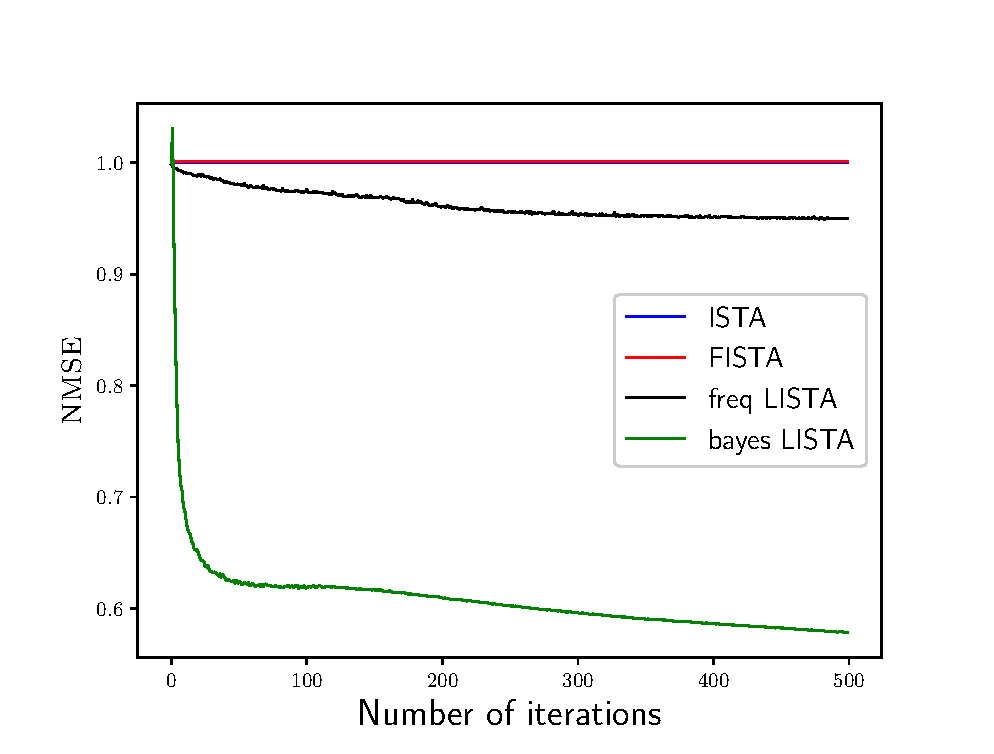
\includegraphics[width=0.5\columnwidth]{graphics/mnist/100_non_normalised_nmse_valid}}

%\begin{figure}[t]
%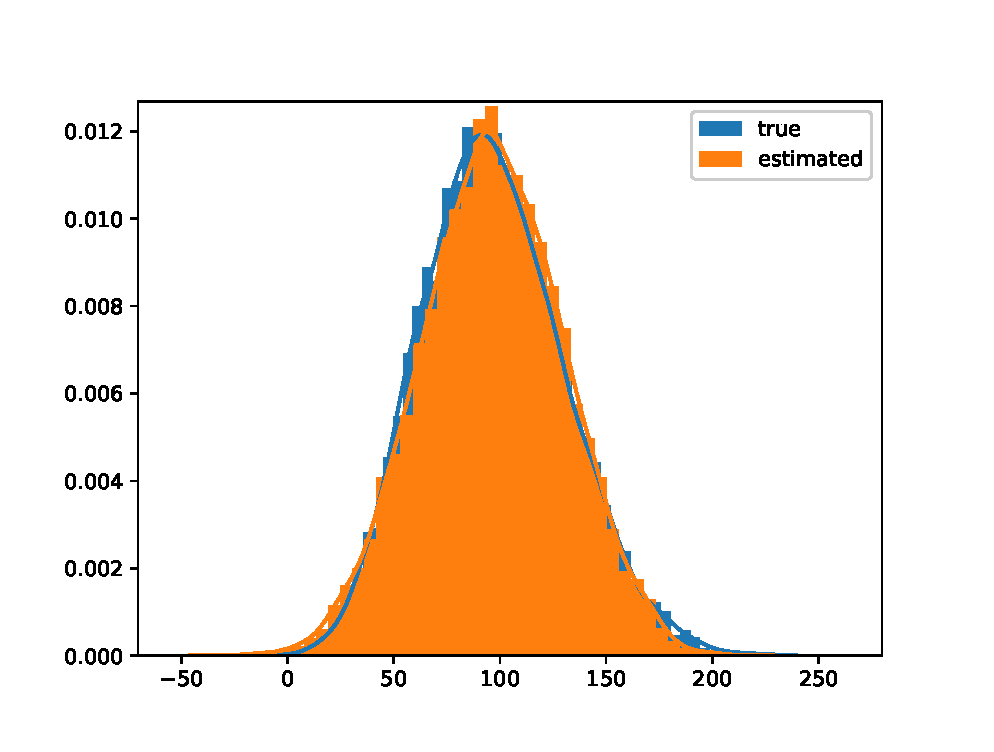
\includegraphics[width=\columnwidth]{d_testing}
%\caption{Approximation of product of Gaussians.}
%\label{fig:d_testing}
%\end{figure}
%
%\begin{figure}[t]
%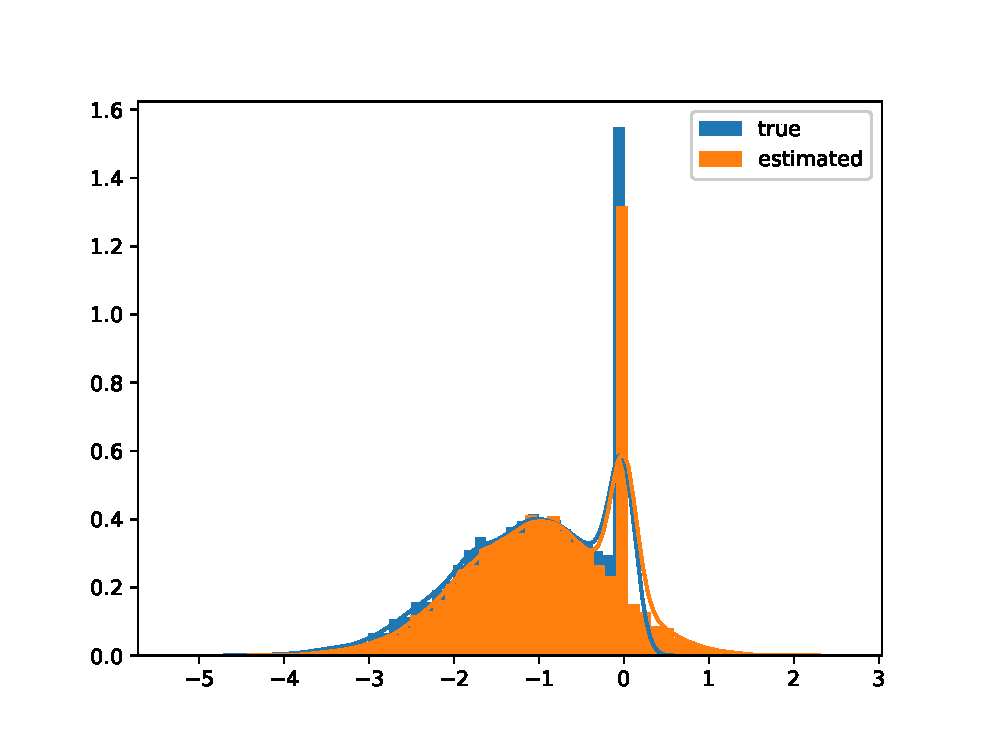
\includegraphics[width=\columnwidth]{z_new_testing}
%\caption{Approximation of propagation through soft thresholding}
%\label{fig:z_new_testing}
%\end{figure}


\section{Backpropagation}
\label{sec:backpropagation}

The exact intractable posterior (\ref{eq:posterior}) is approximated with a factorised distribution
\begin{align}
\label{eq:approximating_dsitribution}
\begin{split}
q(\mathbf{W}, \mathbf{S}, \gamma, \eta) &= \prod_{d=1}^D\prod_{k=1}^K \mathcal{N}(w_{dk} ; m^w_{dk}, v^w_{dk}) \prod_{d'=1}^D\prod_{d''=1}^D \mathcal{N}(s_{d'd''} ; m^s_{d'd''}, v^s_{d'd''}) \\
&\times \text{Gam}(\gamma; a^\gamma, b^\gamma) \text{Gam}(\eta; a^\eta, b^\eta)
\end{split}
\end{align}

For Bayesian inference we expand the probabilistic backpropagation algorithm~\citep{hernandez2015probabilistic} for computing parameter updates. It is based on assumed density filtering (ADF) and expectation propagation (EP) and allows to update parameters of the distributions based on the derivatives of the logarithm of a normalisation constant. ADF iteratively incorporates factors from the true posterior $p$ (\ref{eq:posterior}) into the factorised approximating distribution $q$ (\ref{eq:approximating_dsitribution}), whereas in EP factors in the $q$ are iteratively replaced by factors from $p$.

When a factor from $p$ is incorporated into $q$, $q$ as a function of weights $\mathbf{W}$ and $\mathbf{S}$ has the form:
\begin{equation}
q(a) = Z^{-1}f(a)\mathcal{N}(a; m, v)
\end{equation}
where $Z$ is the normalisation constant and $f(a)$ is an arbitrary function, $a \in \{w_{dk}, s_{d'd''}\}$.

According to \cite{minka2001thesis}, new parameters of the Gaussian distribution for $a$ can be computed as
\begin{equation}
\label{eq:param_update}
m^{\text{new}} = m + v \frac{\partial \log Z}{\partial m}, \qquad
v^{\text{new}} = v - v^2\left[ \left(\frac{\partial \log Z}{\partial m}\right)^2 - 2 \frac{\partial \log Z}{\partial v}\right]
\end{equation}

Then to find new values of $\mathbf{W}$ and $\mathbf{S}$ we need to compute derivatives of the logarithm of $Z$ when the factor of the true posterior $p$ is incorporated in $q$.

With the likelihood factors~(\ref{eq:likelihood}) of the true posterior we employ the ADF approach and iteratively incorporate them into the approximating distribution $q$. The normalisation constant of the approximating distribution $q$ with the likelihood term for the data point $n$ incorporated can be computed as follows (to simplify notation the superscript $(n)$ is omitted)
\begin{align}
Z & = \int \prod_{d=1}^{D} \mathcal{N}(\beta_d ; f(\mathbf{y} ; \mathbf{S}, \mathbf{W}, \lambda), \gamma^{-1}) q(\mathbf{W}, \mathbf{S}, \gamma, \eta) \mathrm{d}\mathbf{W} \mathrm{d}\mathbf{S} \mathrm{d}\gamma \mathrm{d}\eta \nonumber\\
\label{eq:Z}
& \approx \prod_{d=1}^D \left[\omega^{\widehat{\boldsymbol\beta}}_d  \mathcal{T}\left(\beta_d ; 0, \beta^\gamma / \alpha^\gamma, 2\alpha^\gamma\right) + \vphantom{m^{\widehat{\boldsymbol\beta}}_d} \left(1 - \omega^{\widehat{\boldsymbol\beta}}_d\right)\mathcal{N}\left(\beta_d ; m^{\widehat{\boldsymbol\beta}}_d,  \beta^\gamma / (\alpha^\gamma - 1) + v^{\widehat{\boldsymbol\beta}}_d\right)\right].
\end{align}
Parameters of the approximating posterior distribution are then updated with the derivatives of this normalisation constant according to (\ref{eq:param_update}).

Prior factors from $p$ (\ref{eq:ws}), (\ref{eq:gamma_eta}) are incorporated into $q$ with the EP algorithm~\citep{hernandez2015probabilistic}, i.e. they replace the corresponding approximating factors from $q$ and then $q$ is updated to minimise the KL divergence.

\section{Experiments}
\label{sec:experiments}
The proposed Bayesian \textsc{lista} is evaluated in the context of the sparse coding problem with an overcomplete dictionary, where the number of measurements $K$ is much smaller than the dimensionality of the vector $\boldsymbol\beta$.

We compare the proposed Bayesian \textsc{lista} with the classical \textsc{lista}~\citep{gregor2010learning} in terms of the predictive accuracy. As baselines we also use the \textsc{ista} \citep{daubechies2004iterative} and Fast \textsc{ista} (\textsc{fista}) \citep{beck2009fast}. The \textsc{fista} adds the momentum to the \textsc{ista} and improves its convergence speed. We set the number of iterations in these algorithms and the number of layers in the Bayesian and classical \textsc{lista} networks to $L$. To measure the performance of the algorithms the normalised mean square error (\textsc{nmse}) and F measure are used. We demonstrate the performance on small datasets to highlight that the proposed algorithm can infer accurate predictions when the dataset size is not sufficient for the \textsc{lista} to learn.

\begin{figure}[t!]
\centering
%\subfloat[\textsc{nmse} on train]{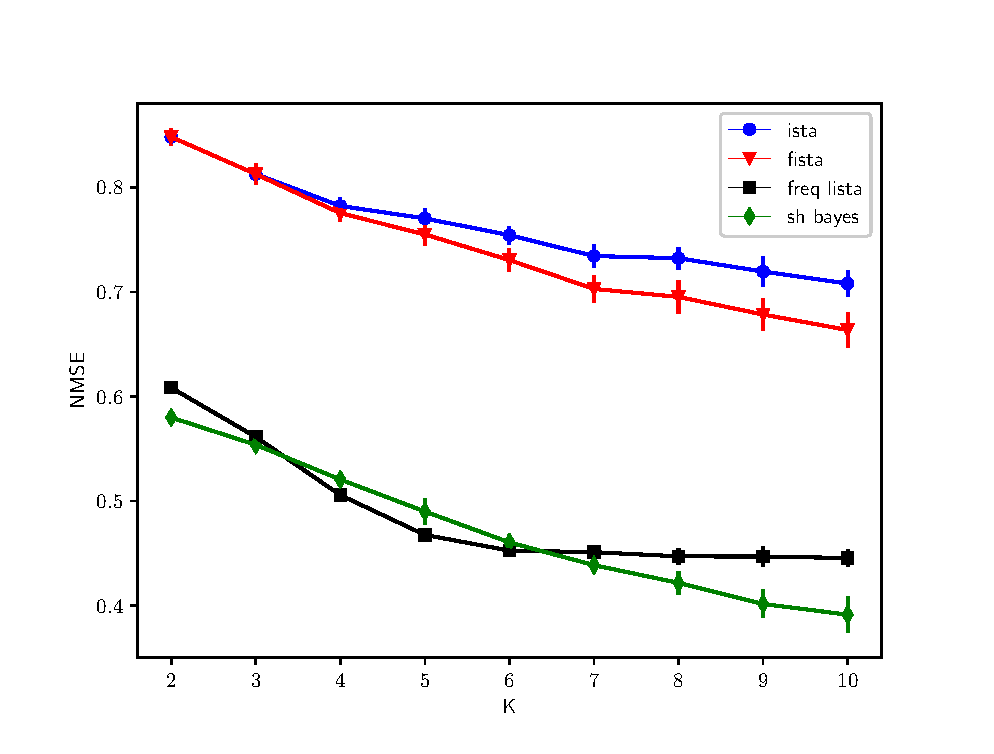
\includegraphics[width=0.5\columnwidth]{graphics/synthetic_number_of_layers/nmse_train}}
%~
\subfloat[\textsc{nmse} for different $L$]{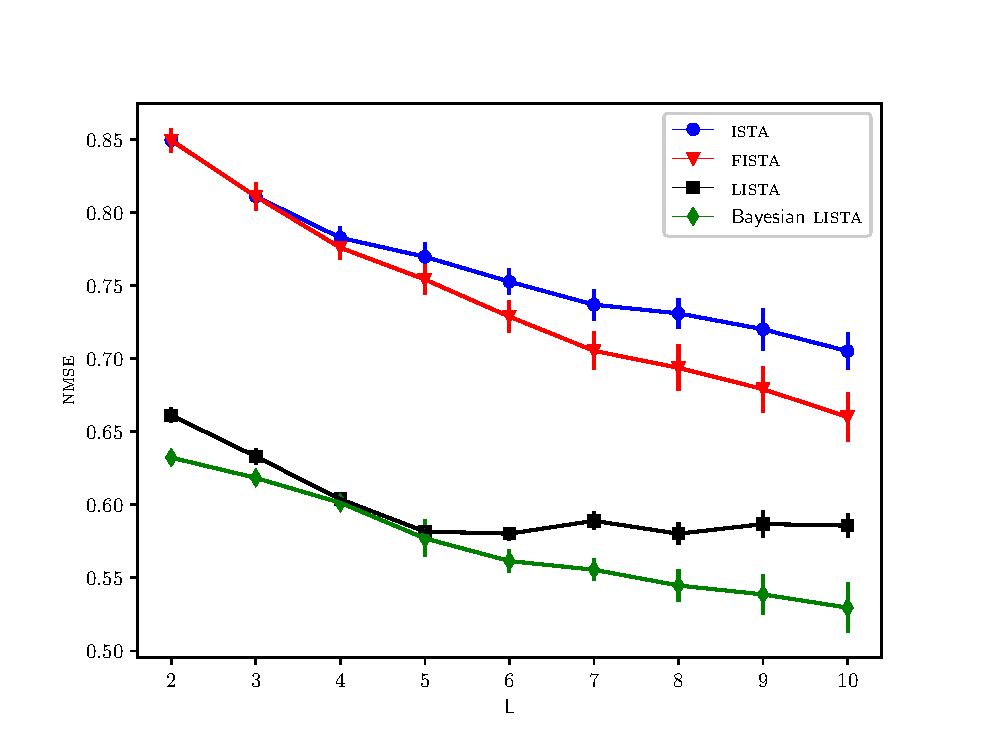
\includegraphics[width=0.4\columnwidth]{graphics/synthetic_number_of_layers/nmse_validation}
\label{fig:nmse_n_layers_synthetic}}
%\subfloat[F measure on train]{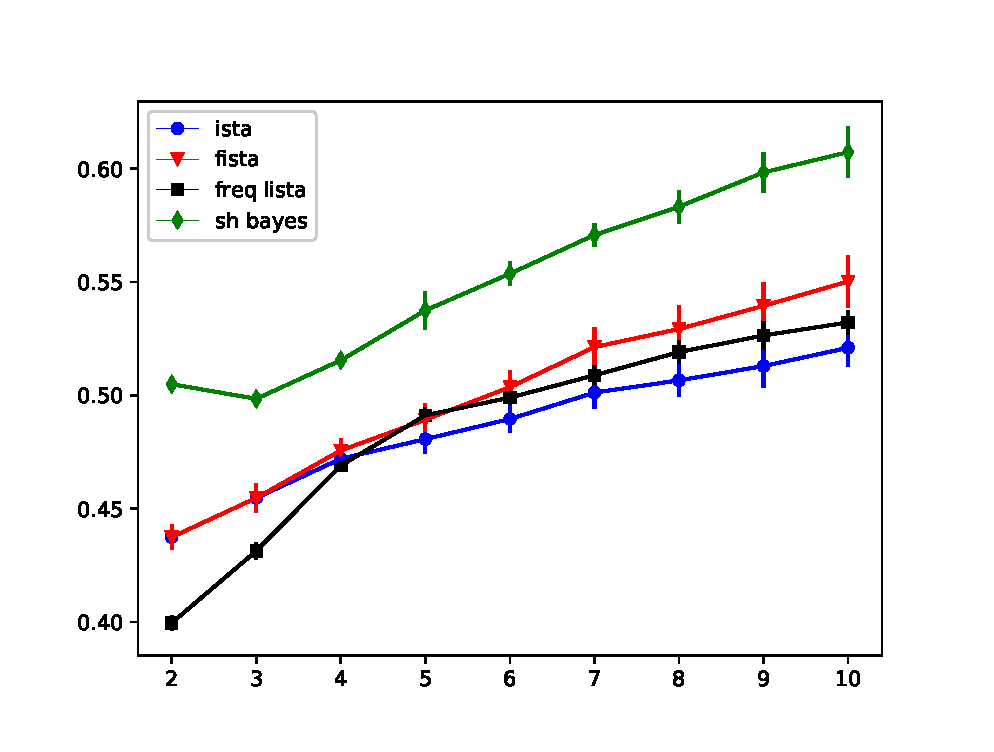
\includegraphics[width=0.5\columnwidth]{graphics/synthetic_number_of_layers/f_measure_train}}
%~
\subfloat[F measure for different $L$]{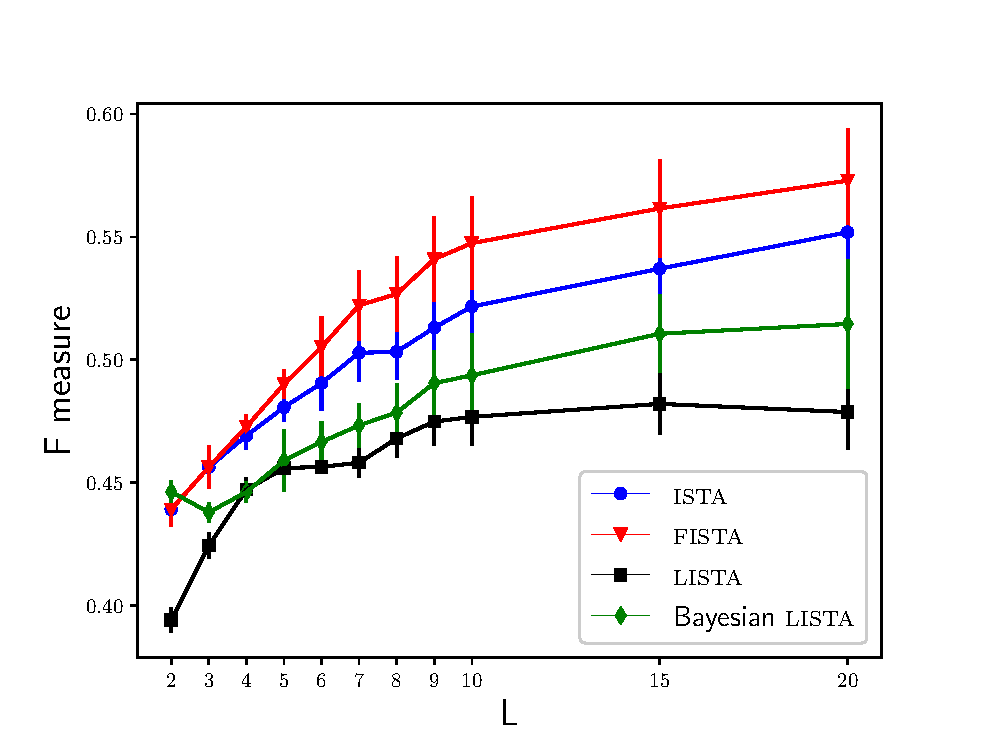
\includegraphics[width=0.4\columnwidth]{graphics/synthetic_number_of_layers/f_measure_validation}
\label{fig:f_meas_n_layers_synthetic}}\\[-13pt]
\subfloat[\textsc{nmse} for different $K$]{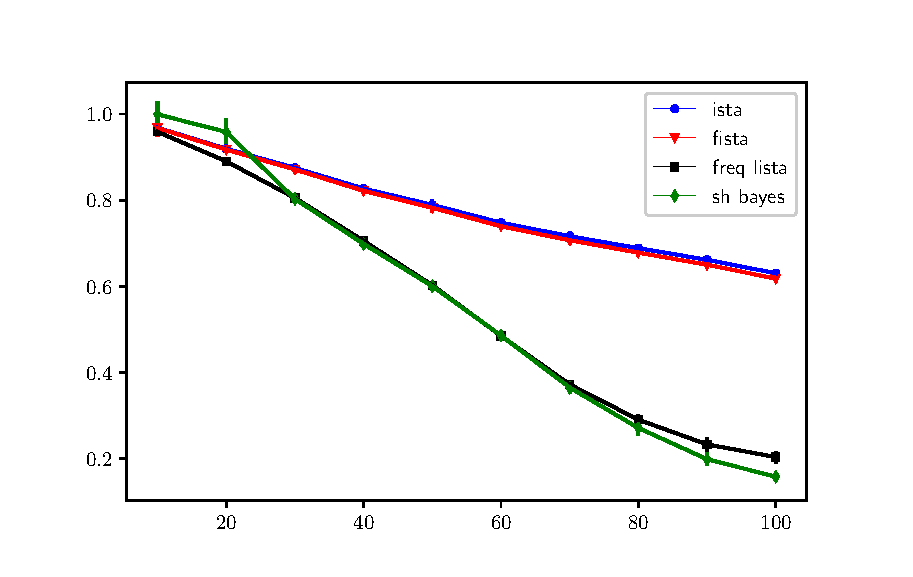
\includegraphics[width=0.4\columnwidth]{graphics/synthetic_undersampling/nmse_validation}
\label{fig:nmse_undersampling_synthetic}}
%\subfloat[F measure on train]{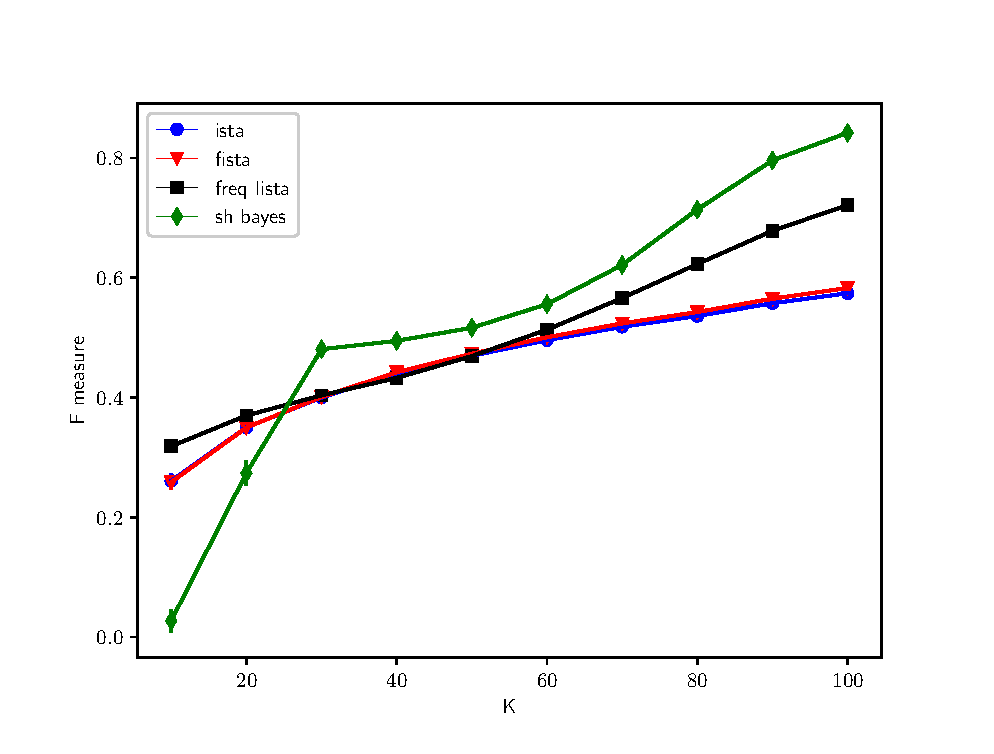
\includegraphics[width=0.5\columnwidth]{graphics/synthetic_undersampling/f_measure_train}}
%~
\subfloat[F measure for different $K$]{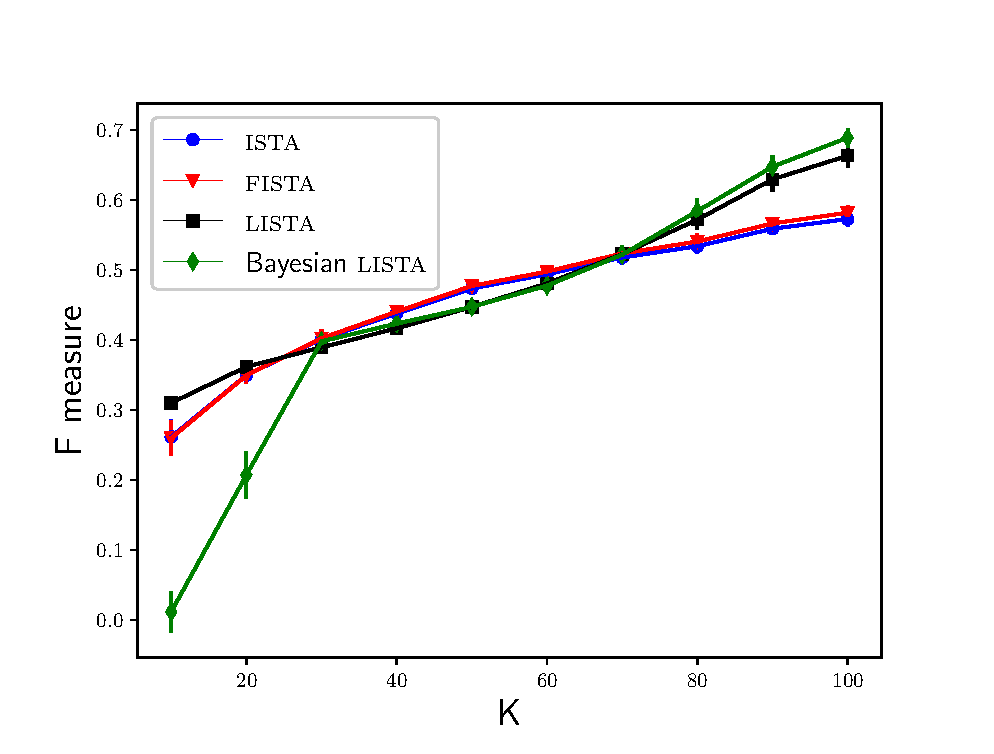
\includegraphics[width=0.4\columnwidth]{graphics/synthetic_undersampling/f_measure_validation}
\label{fig:f_meas_undesampling_synthetic}}
\caption{Predictive accuracy on the synthetic data: the top row for different numbers of layers (for neural networks) or iterations (for baselines),  the bottom row for different sizes of observations}
\label{fig:number_of_layers_synthetic}
\end{figure}

\subsection{Predictive performance on synthetic data}
First, the predictive performance of the proposed Bayesian \textsc{lista} is analysed on synthetic data. We generate $N_\text{train}=1000$ and $N_{\text{test}} = 100$ sparse coefficients vectors $\boldsymbol\beta^{(n)}$ each of size $D = 100$. Coefficients $\boldsymbol\beta^{(n)}$ are generated from the spike and slab distribution with the truncated slab: each component $\beta^{(n)}_{d}$ is zero with the probability $0.8$ or is from the standard Gaussian distribution without interval $(-0.1, 0.1)$ with the probability $0.2$. To simulate sparse observations, we generate the random Gaussian design matrix $\mathbf{X} \in \mathbb{R}^{K \times D}$.  The observations are generated according to (\ref{eq:regression_problem}) with the zero-mean Gaussian noise with the standard deviation $0.5$. The shrinkage parameter is set to~$\lambda = 0.1$. We train the algorithms using the training data of size $N_\text{train}$ and measure performance on the test data of size $N_{\text{test}}$.

In Figures \ref{fig:nmse_n_layers_synthetic} and \ref{fig:f_meas_n_layers_synthetic} predictive performance for different number of layers $L$ is presented. The observation size is set to $K=50$. The Bayesian \textsc{lista} outperforms the \textsc{lista} in terms of both measures. Although the baselines \textsc{ista} and \textsc{fista} show better performance in terms of F measure, the Bayesian \textsc{lista} has the lowest \textsc{nmse}.

Figures~\ref{fig:nmse_undersampling_synthetic} and~\ref{fig:f_meas_undesampling_synthetic} give the results of predictive performance for different observation sizes $K$. The number of layers is set as $L=4$. In the previous experiment the Bayesian and classical \textsc{lista} show similar results with this number of layers. The results of Figures~\ref{fig:nmse_undersampling_synthetic} and~\ref{fig:f_meas_undesampling_synthetic} confirm this competitive behaviour between two \textsc{lista} networks. Baselines show similar results in terms of F measure and underperform in terms of \textsc{nmse}. Overall, the experiments on the synthetic data demonstrate that the Bayesian \textsc{lista} provides competitive results in terms of predictive accuracy.

%We compare two versions of the proposed Bayesian LISTA: with shared weight matrices and with individual matrices at each layer --- and LISTA.

%The NMSE is presented in figure \ref{fig:validation_synthetic}.
%\begin{figure}[t]
%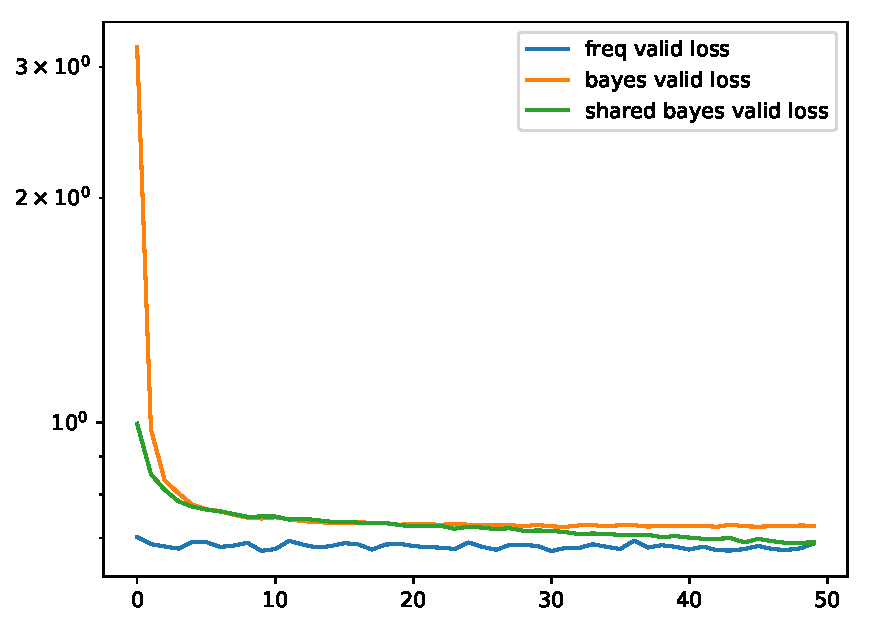
\includegraphics[width=\columnwidth]{loss_synthetic}
%\caption{Validation NMSE on synthetic data}
%\label{fig:validation_synthetic}
%\end{figure}

\begin{figure}[t!]
\centering
%\subfloat[\textsc{nmse} on train]{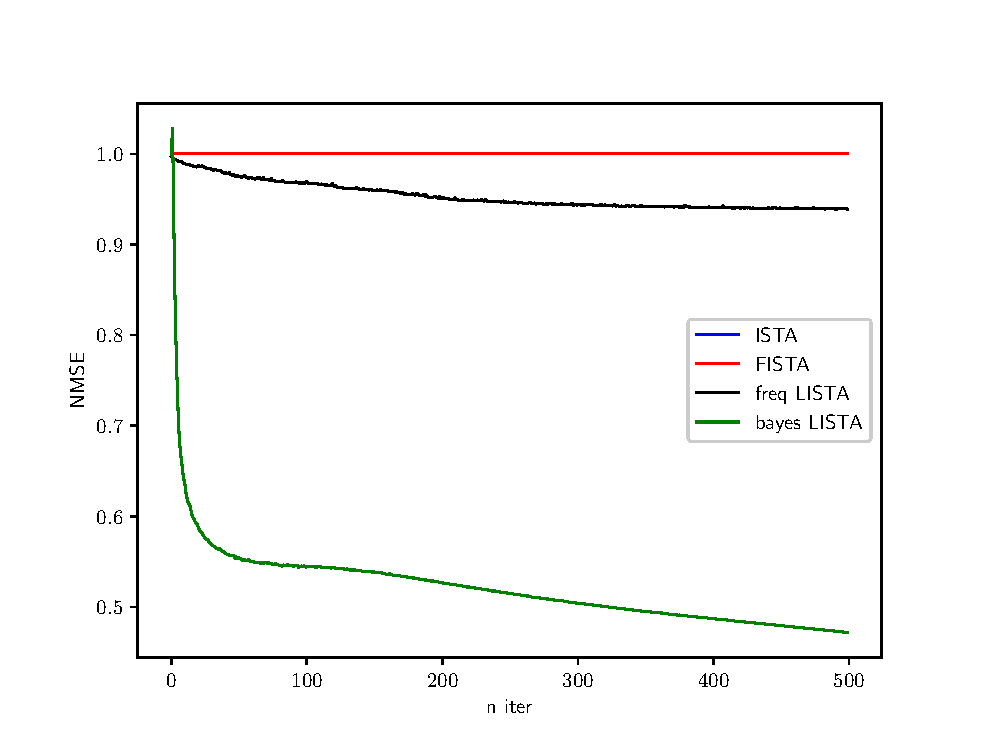
\includegraphics[width=0.5\columnwidth]{graphics/mnist/100_normalised_nmse_train}}
%~
\subfloat[\textsc{nmse} for $K = 100$]{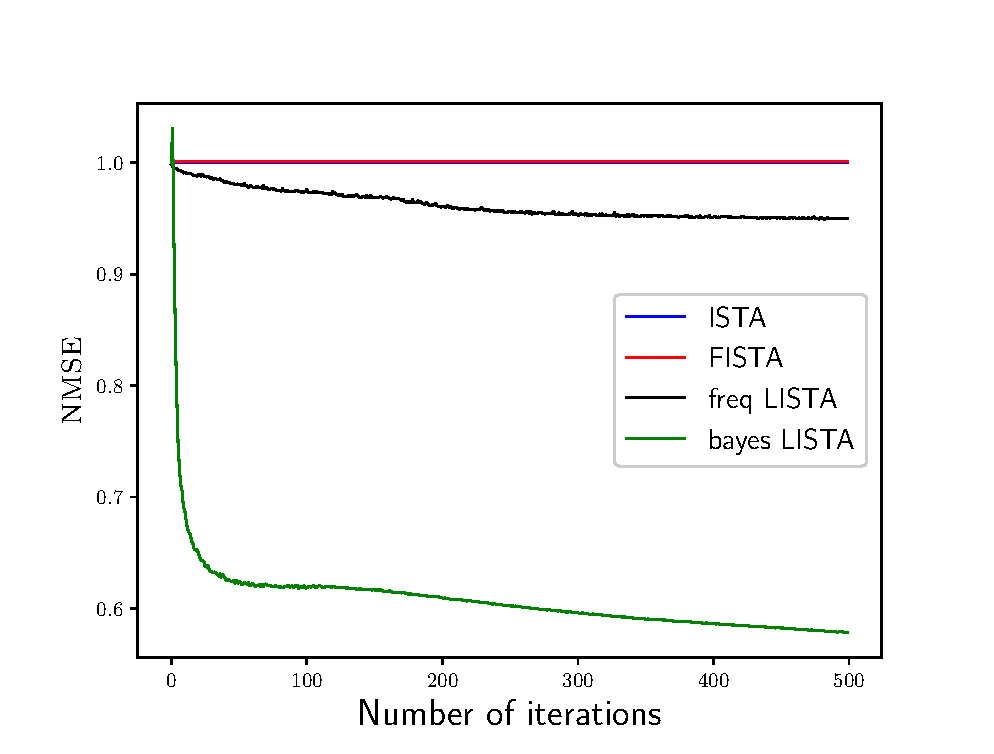
\includegraphics[width=0.4\columnwidth]{graphics/mnist/100_non_normalised_nmse_valid}}
%\subfloat[F measure on train]{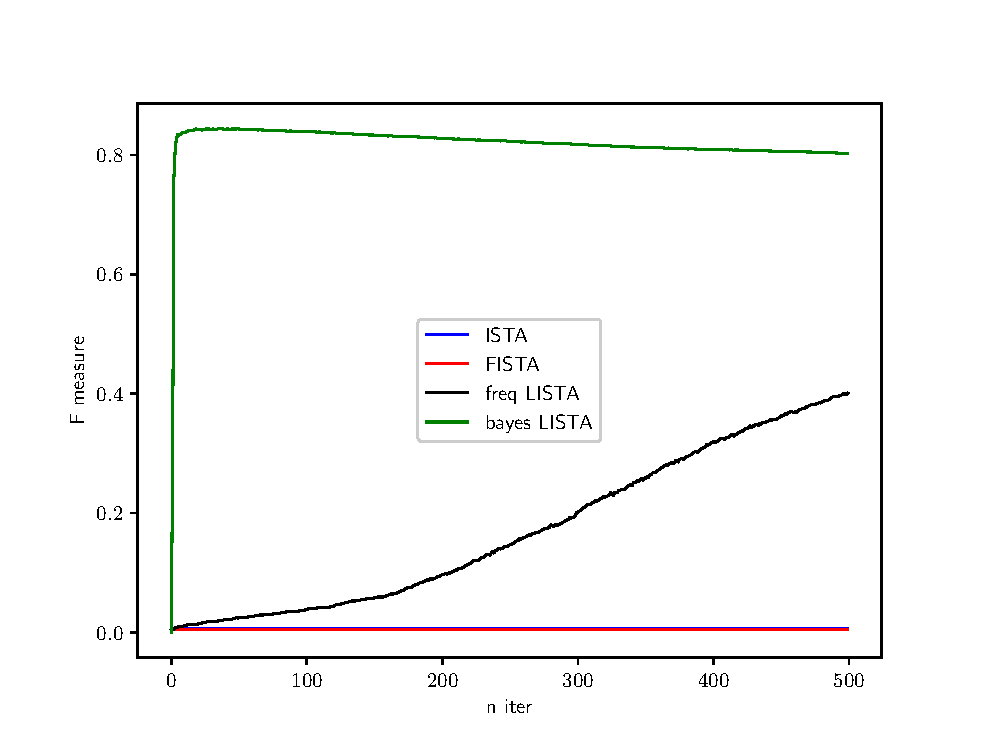
\includegraphics[width=0.5\columnwidth]{graphics/mnist/100_normalised_f_measure_train}}
%~
\subfloat[F measure for $K = 100$]{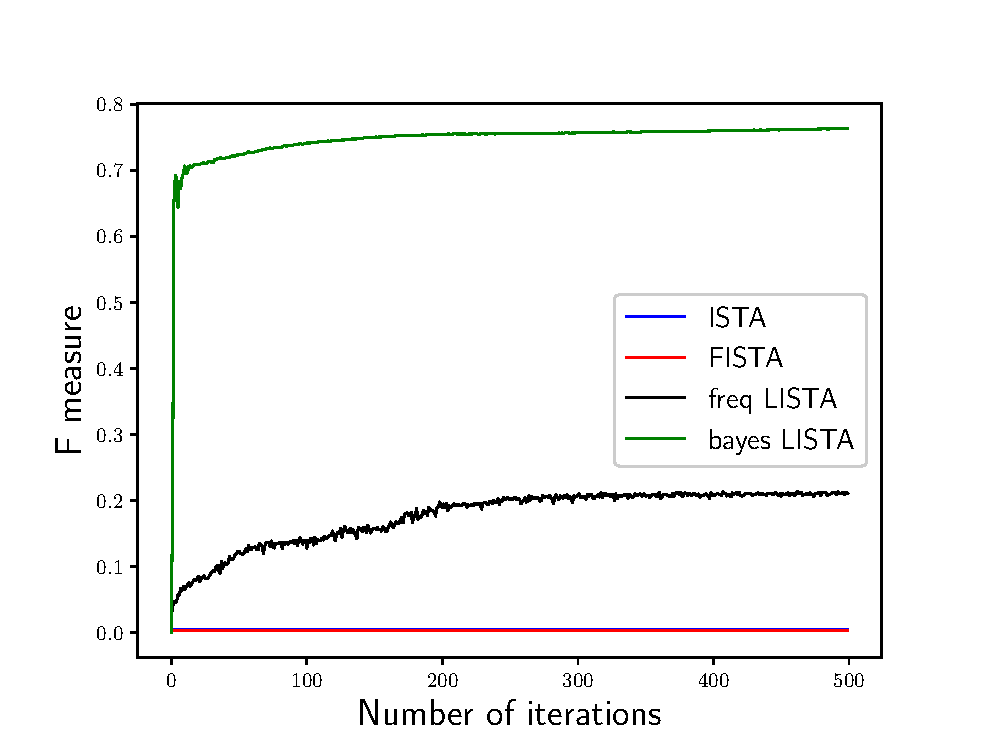
\includegraphics[width=0.4\columnwidth]{graphics/mnist/100_non_normalised_f_measure_valid}}\\[-13pt]
\subfloat[\textsc{nmse} for $K = 250$]{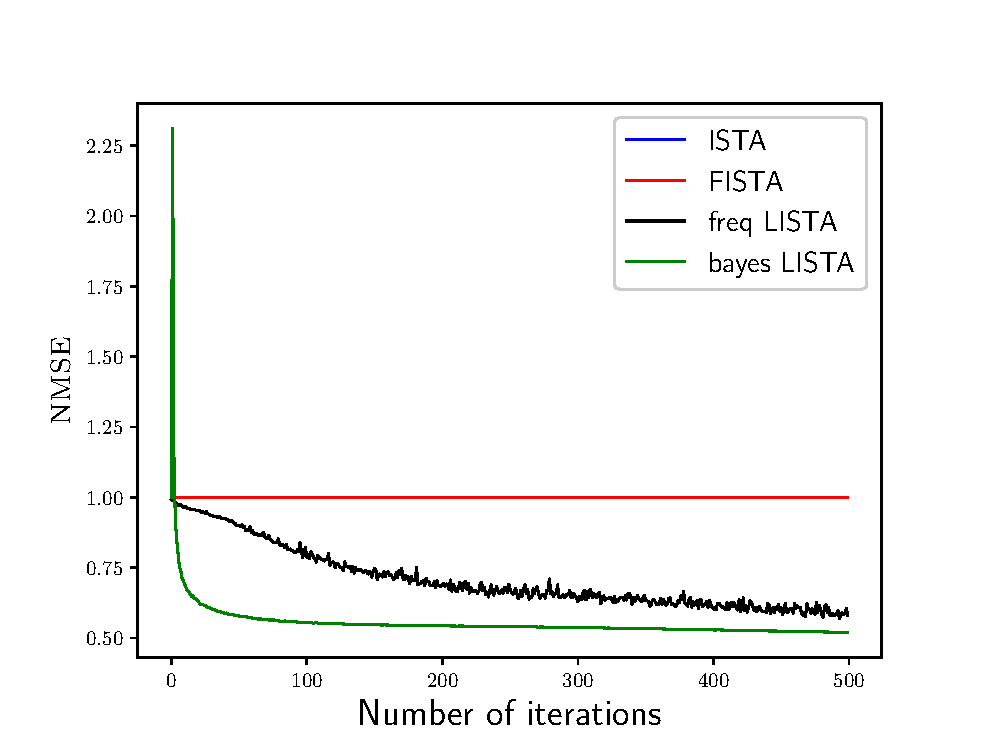
\includegraphics[width=0.4\columnwidth]{graphics/mnist/250_non_normalised_nmse_valid}}
%\subfloat[F measure on train]{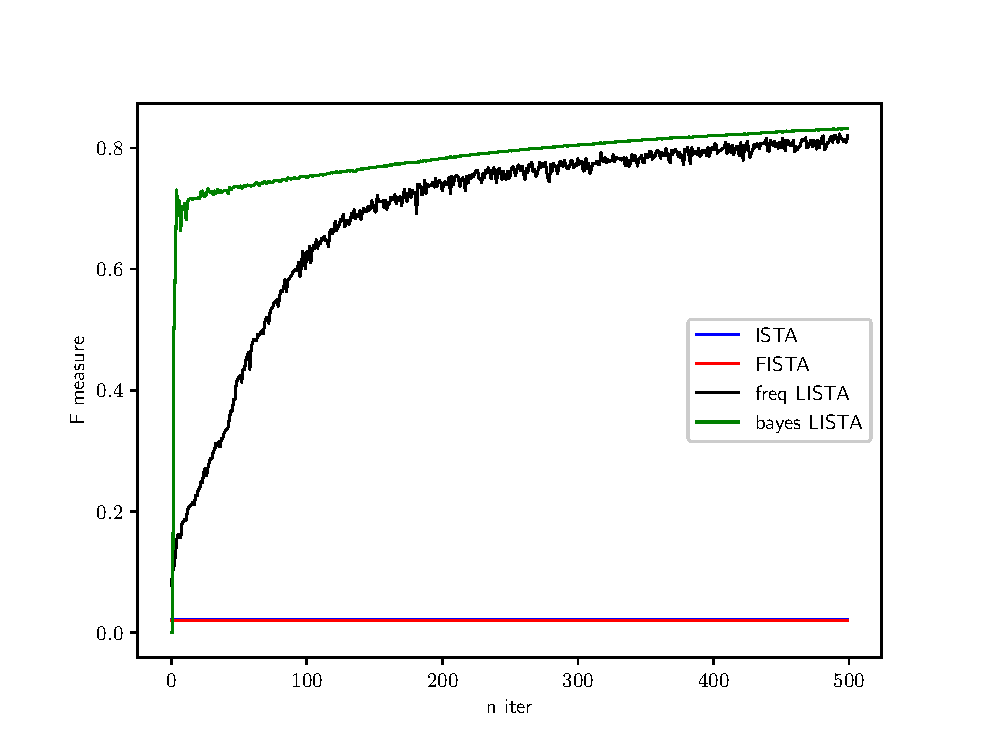
\includegraphics[width=0.5\columnwidth]{graphics/mnist/250_normalised_f_measure_train}}
%~
\subfloat[F measure for $K = 250$]{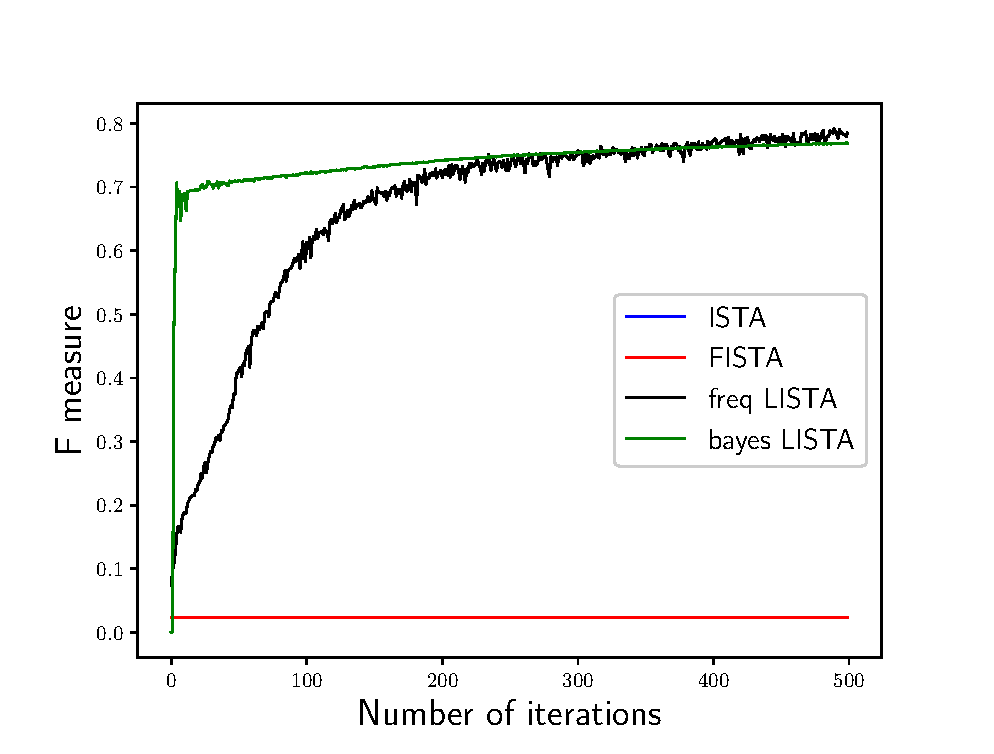
\includegraphics[width=0.4\columnwidth]{graphics/mnist/250_non_normalised_f_measure_valid}}
\caption{Predictive performance for different numbers of iterations on the \textsc{mnist} data with the dictionary size $K = 100$ (the top row) and $K = 250$ (the bottom row)}
\label{fig:mnist}
\end{figure}

\subsection{Predictive performance on \textsc{mnist} data}
Here we evaluate the proposed Bayesian \textsc{lista} in terms of predictive performance on the \textsc{mnist} dataset \citep{lecun1998gradient}. The dataset contains images of handwritten digits of size $28 \times 28 = 784$. The design matrix $\mathbf{X}$ is generated as standard random Gaussian. The resulting size of $\mathbf{X}$ is $K \times 784$. Then we generate observations as $\mathbf{y} = \mathbf{X}\boldsymbol\beta$, where $\boldsymbol\beta \in \mathbb{R}^{784}$ are flatten images. We use $100$ images for training and $100$ for test. The shrinkage parameter $\lambda$ is fixed as $0.1$.

Figure \ref{fig:mnist} present quality on the validation set with dictionaries of size $100$ and $250$.  The experiment with $K=100$ presents severe conditions for the algorithms: the very limited size of the training dataset combined with the small dimensionality of observations. The Bayesian \textsc{lista} is able to learn under these conditions, outperforming the \textsc{lista} that demonstrates poor results. Under better conditions of the second experiment with $K=250$ both \textsc{lista} networks converge to the similar results. However, the Bayesian \textsc{lista} demonstrates remarkably better convergence rate. Both baselines are unable to perform well in these experiments. The proposed Bayesian \textsc{lista} network also estimates the posterior distribution for $\boldsymbol\beta$. The parameters of the posterior distribution and samples from it are given in the supplementary materials.

\subsection{Active learning}
To demonstrate a potential scenario that can benefit from uncertainty estimates of the Bayesian \textsc{lista} we consider the active learning example \citep{settles.tr09}. The active learning area researches ways to select new training subsets to reduce the total number of required supervision. One of the popular approaches in active learning is uncertainty sampling when the data with the least certain predictions is chosen to obtain a new label at. Uncertainty is usually measured with entropy. In our case of the spike and slab distributed data points there is no closed form for entropy. Therefore, we use a variance from Lemma~\ref{thm:moments_spsl} as a measure of uncertainty.

The data in this example is the \textsc{mnist} dataset with the learnt dictionary of size $K=100$. We use the training data of size $50$, the pool data of size $500$,  and the test data of size $100$. The algorithm learns on the training data for $50$ iterations and it is evaluated on the test data. To actively collect a next data point from the pool, the algorithm is used to predict a point with the highest uncertainty. The selected point is moved from the pool to the training data and the algorithm performs additional $10$ iterations on the updated training data. Overall, $10$ pool additions are performed. After every addition the performance is measured on the test data. We compare the actively updated approach of adding new points from the pool with the random approach that picks a new data point from the pool at random. The procedure is repeated for $20$ times with new randomly selected initial datasets.

Figure \ref{fig:active_learning_mnist} demonstrates performance of the active and non-active methods of updates with the Bayesian \textsc{lista}. The active approach with uncertainty sampling steadily demonstrates better results in terms of both quality measures. This means that the posterior distribution learnt by the Bayesian \textsc{lista} is an adequate estimate of the true posterior.
\begin{figure}[t]
\centering
\subfloat[\textsc{nmse}]{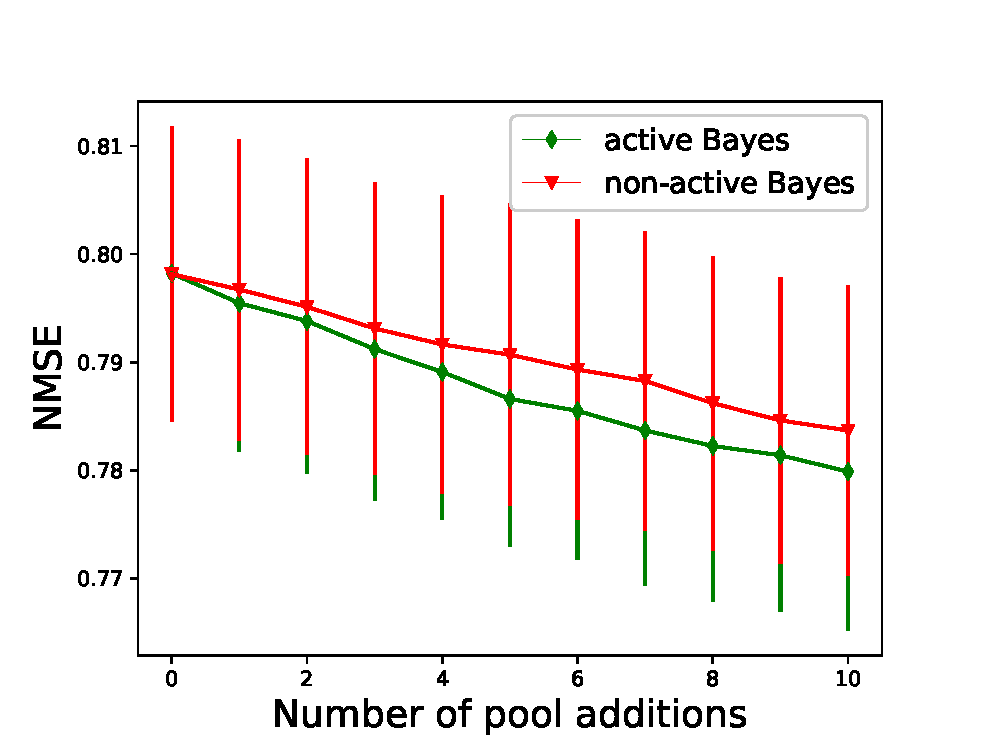
\includegraphics[width=0.4\columnwidth]{graphics/active_mnist/nmse_validation}}%
\subfloat[F measure]{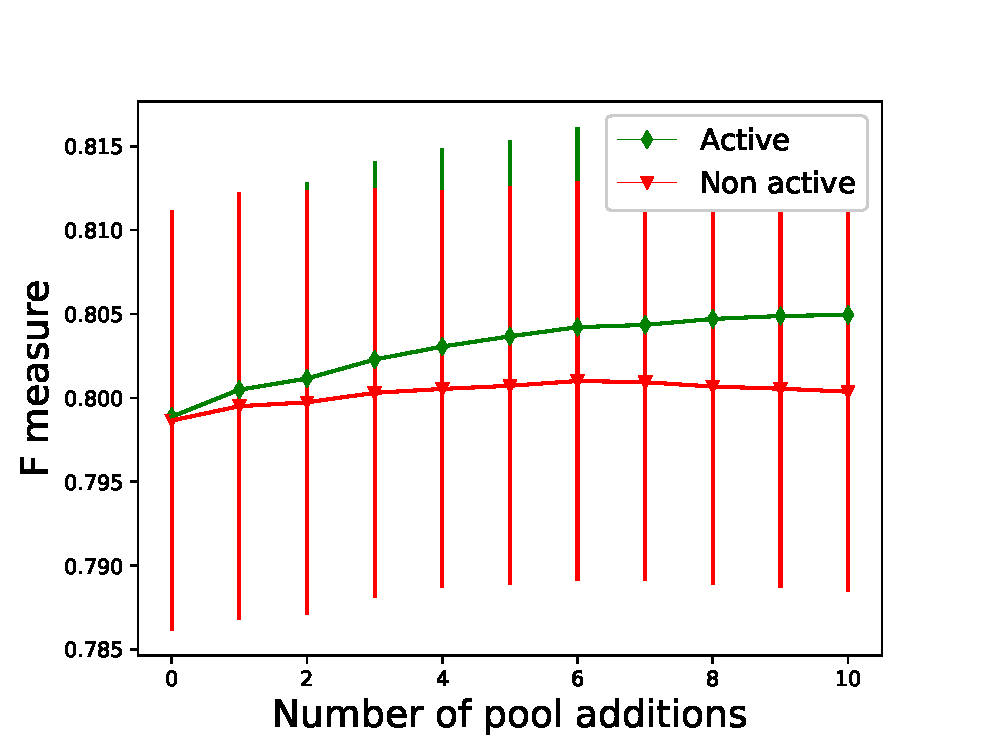
\includegraphics[width=0.4\columnwidth]{graphics/active_mnist/f_measure_validation}}
\caption{Performance for the active learning experiment on the \textsc{mnist} data. }
\label{fig:active_learning_mnist}
\end{figure}

\section{Discussion}
\label{sec:discussion}
To the best of our knowledge, this is the first implementation of a Bayesian deep sparse coding algorithm. Although there are works on Bayesian sparsity in context of neural networks \citep{he2017bayesian}, they are not the Bayesian neural networks in the same sense as the Bayesian \textsc{lista} but rather the interpretation of the sparse Bayesian  learning algorithm as the long short-term memory network. We find not only correct predictions but also useful posterior estimates for the predictions.

%The inference is based on the expectation propagation algorithm and though it is not suited for distributed inference, stochastic variant of assumed density filtering can potentially be used \citep{li2015stochastic}. This would allow the proposed approach to scale.

The \textsc{lista}-based algorithms can be applied for the sparse coding problem with both overcomplete (i.e., $D > K$) as in the original paper \citep{gregor2010learning}, and undercomplete (i.e., $D < K$) dictionaries. Section~\ref{sec:experiments} provides experiments for the overcomplete case, we give experiments for the undercomplete case in the supplementary material.

\section{Conclusions and future work}
\label{sec:conclusions}
We have presented the new method for propagating uncertainty through the soft thresholding function. %To achieve this goal
We have approximated the outputs of the function with a spike and slab distribution, and we have shown that this distribution can stay within the same family after linear transformation with Gaussian weights and inputs of a neural network. This allowed us to propose the Bayesian \textsc{lista} network and efficient inference algorithm that learns the distributions of the weights and makes the uncertainty estimates of the outputs. The forward propagation in the algorithm is based on the proposed uncertainty propagation method, the backward propagation is based on the probabilistic backpropagation method, that was remarkably expanded to account for multidimensionality of inputs and outputs, likelihood of the Bayesian \textsc{lista} and its recurrent nature.

Experiments on the synthetic and \textsc{mnist} datasets demonstrate that the proposed algorithm preserves the predictive accuracy of non-Bayesian methods while also providing posterior estimates. We also show that when the training data is very small the proposed algorithm significantly outperforms the classical \textsc{lista} in terms of predictive accuracy. Experiments on active learning demonstrate that the proposed Bayesian \textsc{lista} gives accurate posterior estimates that can be used for selection of a next data point where a label should be obtain at.

The shrinkage parameter $\lambda$ is currently treated as a deterministic hyperparameter for the Bayesian \textsc{lista}. In future we plan to incorporate it into the model treating it as a random variable. For this we will extend both the uncertainty propagation method to include uncertainty of $\lambda$ and the probabilistic backpropagation algorithm to estimate its posterior. We will study stochastic expectation propagation applicability in order to replace ADF that may further improve the quality of posterior estimates~\citep{li2015stochastic}.

\bibliography{bibliography}
\bibliographystyle{icml2018}

\end{document}
